% Verze pro: LaTeX
% Verze hlavicky: 22. 2. 2007
% Autor: Ustav fyziky kondenzovanych latek
% Ke stazeni: www.physics.muni.cz/ufkl/Vyuka/
% Licence: volne k pouziti, nejlepe k vcasnemu odevzdani protokolu z Vaseho mereni.

\documentclass[a4paper,11pt]{article}

% Kodovani (cestiny) v dokumentu: cp1250
% \usepackage[cp1250]{inputenc}	% Omezena stredoevropska kodova stranka, pouze MSW.
\usepackage[utf8]{inputenc}	% Doporucujeme pouzivat UTF-8 (unicode).

%%% Nemente:
\usepackage[margin=2cm]{geometry}
\newtoks\jmenopraktika \newtoks\jmeno \newtoks\datum
\newtoks\obor \newtoks\skupina \newtoks\rocnik \newtoks\semestr
\newtoks\cisloulohy \newtoks\jmenoulohy
\newtoks\tlak \newtoks\teplota \newtoks\vlhkost
%%% Nemente - konec.


%%%%%%%%%%% Doplnte pozadovane polozky:

\jmenopraktika={Fyzikální praktikum 1}  % nahradte jmenem vaseho predmetu
\jmeno={Milan Suk}            % nahradte jmenem mericiho
\datum={9. března 2017}        % nahradte datem mereni ulohy
\obor={F}                     % nahradte zkratkou vami studovaneho oboru
\skupina={ČT 8:00}            % nahradte dobou vyuky vasi seminarni skupiny
\rocnik={I}                  % nahradte rocnikem, ve kterem studujete
\semestr={II}                 % nahradte semestrem, ve kterem studujete

\cisloulohy={5}               % nahradte cislem merene ulohy
\jmenoulohy={Měření modulu pružnosti pevných látek} % nahradte jmenem merene ulohy

\tlak={99,9}                   % nahradte tlakem pri mereni (v hPa)
\teplota={23,8}               % nahradte teplotou pri mereni (ve stupnich Celsia)
\vlhkost={45}               % nahradte vlhkosti vzduchu pri mereni (v %)

%%%%%%%%%%% Konec pozadovanych polozek.


%%%%%%%%%%% Uzitecne balicky:
\usepackage[czech]{babel}
\usepackage{graphicx}
\usepackage{amsmath}
\usepackage{xspace}
\usepackage{url}
\usepackage{indentfirst}

%%%%%% Zamezeni parchantu:
\widowpenalty 10000 \clubpenalty 10000 \displaywidowpenalty 10000
%%%%%% Parametry pro moznost vsazeni vetsiho poctu obrazku na stranku
\setcounter{topnumber}{3}	  % max. pocet floatu nahore (specifikace t)
\setcounter{bottomnumber}{3}	  % max. pocet floatu dole (specifikace b)
\setcounter{totalnumber}{6}	  % max. pocet floatu na strance celkem
\renewcommand\topfraction{0.9}	  % max podil stranky pro floaty nahore
\renewcommand\bottomfraction{0.9} % max podil stranky pro floaty dole
\renewcommand\textfraction{0.1}	  % min podil stranky, ktery musi obsahovat text
\intextsep=8mm \textfloatsep=8mm  %\intextsep pro ulozeni [h] floatu a \textfloatsep pro [b] or [t]

% Tecky za cisly sekci:
\renewcommand{\thesection}{\arabic{section}.}
\renewcommand{\thesubsection}{\thesection\arabic{subsection}.}
% Jednopismenna mezera mezi cislem a nazvem kapitoly:
\makeatletter \def\@seccntformat#1{\csname the#1\endcsname\hspace{1ex}} \makeatother


%%%%%%%%%%%%%%%%%%%%%%%%%%%%%%%%%%%%%%%%%%%%%%%%%%%%%%%%%%%%%%%%%%%%%%%%%%%%%%%
%%%%%%%%%%%%%%%%%%%%%%%%%%%%%%%%%%%%%%%%%%%%%%%%%%%%%%%%%%%%%%%%%%%%%%%%%%%%%%%
% Zacatek dokumentu
%%%%%%%%%%%%%%%%%%%%%%%%%%%%%%%%%%%%%%%%%%%%%%%%%%%%%%%%%%%%%%%%%%%%%%%%%%%%%%%
%%%%%%%%%%%%%%%%%%%%%%%%%%%%%%%%%%%%%%%%%%%%%%%%%%%%%%%%%%%%%%%%%%%%%%%%%%%%%%%

\begin{document}

%%%%%%%%%%%%%%%%%%%%%%%%%%%%%%%%%%%%%%%%%%%%%%%%%%%%%%%%%%%%%%%%%%%%%%%%%%%%%%%
% Nemente:
%%%%%%%%%%%%%%%%%%%%%%%%%%%%%%%%%%%%%%%%%%%%%%%%%%%%%%%%%%%%%%%%%%%%%%%%%%%%%%%
\thispagestyle{empty}

{
\begin{center}
\sf 
{\Large Ústav fyzikální elektroniky Přírodovědecké fakulty Masarykovy univerzity} \\
\bigskip
{\huge \bfseries FYZIKÁLNÍ PRAKTIKUM} \\
\bigskip
{\Large \the\jmenopraktika}
\end{center}

\bigskip

\sf
\noindent
\setlength{\arrayrulewidth}{1pt}
\begin{tabular*}{\textwidth}{@{\extracolsep{\fill}} l l}
\large {\bfseries Zpracoval:}  \the\jmeno & \large  {\bfseries Naměřeno:} \the\datum\\[2mm]
\large  {\bfseries Obor:} \the\obor  \hspace{40mm}  {\bfseries Skupina:} \the\skupina %
%{\bfseries Ročník:} \the\rocnik \hspace{5mm} {\bfseries Semestr:} \the\semestr  
&\large {\bfseries Testováno:}\\
\\
\hline
\end{tabular*}
}

\bigskip

{
\sf
\noindent \begin{tabular}{p{3cm} p{0.6\textwidth}}
\Large  Úloha č. {\bfseries \the\cisloulohy:} \par
\smallskip
$T=\the\teplota$~$^\circ$C \par
$p=\the\tlak$~hPa \par
$\varphi=\the\vlhkost$~\%
&\Large \bfseries \the\jmenoulohy  \\[2mm]
\end{tabular}
}

\vskip1cm

%%%%%%%%%%%%%%%%%%%%%%%%%%%%%%%%%%%%%%%%%%%%%%%%%%%%%%%%%%%%%%%%%%%%%%%%%%%%%%%
% konec Nemente.
%%%%%%%%%%%%%%%%%%%%%%%%%%%%%%%%%%%%%%%%%%%%%%%%%%%%%%%%%%%%%%%%%%%%%%%%%%%%%%%

%%%%%%%%%%%%%%%%%%%%%%%%%%%%%%%%%%%%%%%%%%%%%%%%%%%%%%%%%%%%%%%%%%%%%%%%%%%%%%%
%%%%%%%%%%%%%%%%%%%%%%%%%%%%%%%%%%%%%%%%%%%%%%%%%%%%%%%%%%%%%%%%%%%%%%%%%%%%%%%
% Zacatek textu vlastniho protokolu
%%%%%%%%%%%%%%%%%%%%%%%%%%%%%%%%%%%%%%%%%%%%%%%%%%%%%%%%%%%%%%%%%%%%%%%%%%%%%%%
%%%%%%%%%%%%%%%%%%%%%%%%%%%%%%%%%%%%%%%%%%%%%%%%%%%%%%%%%%%%%%%%%%%%%%%%%%%%%%%


\section{Úvod}

    \paragraph{} Cílem toho měření je změřit
    
    \begin{enumerate}
        \item modul pružnosti v tahu přímou metodou pro ocelový drát zavěšený při stěně
        \item modul pružnosti v tahu z průhybu nosníku
        \item modul pružnosti ve smyku pro ocelový drát dynamickou metodou z torzních kmitů
    \end{enumerate}

\section{Postup měření}

        \begin{table}[h]
            \centering
            \begin{tabular}{ | l || l | l | }
                \hline
                    N & závaží pro 1. měření & závaží pro 2. měření \\ \hline
                    1 & 112.759 & 99.643 \\ \hline
                    2 & 108.130 & 99.643 \\ \hline
                    3 & 112.200 & 98.985 \\ \hline
                    4 & 113.586 & 99.752 \\ \hline
                    5 & 113.163 & 99.771 \\ \hline
                    6 & 112.054 & 99.682 \\ \hline
                    7 & 113.350 & 99.645 \\ \hline
                    8 & 120.120 & 99.385 \\ \hline
                    9 & 108.389 & 99.418 \\ \hline
                    10 & 115.190 & 99.133 \\
                \hline
            \end{tabular}
            \caption{Měření hmotností závaží}
            \label{fig:hmotnosti}
        \end{table}

    \subsection{Modul pružnosti v tahu přímou metodou}

        \paragraph{} Nejprve jsem určil hmotnosti $m_{i}$ zatěžovacích závaží na digitálních váhách.
        Znám délku drátu $l = 1.565m$ a změřil jsem si jeho tloušťku $d = (1.00 \pm 0.01) mm$. 

        \begin{figure}[h]
            \centering
            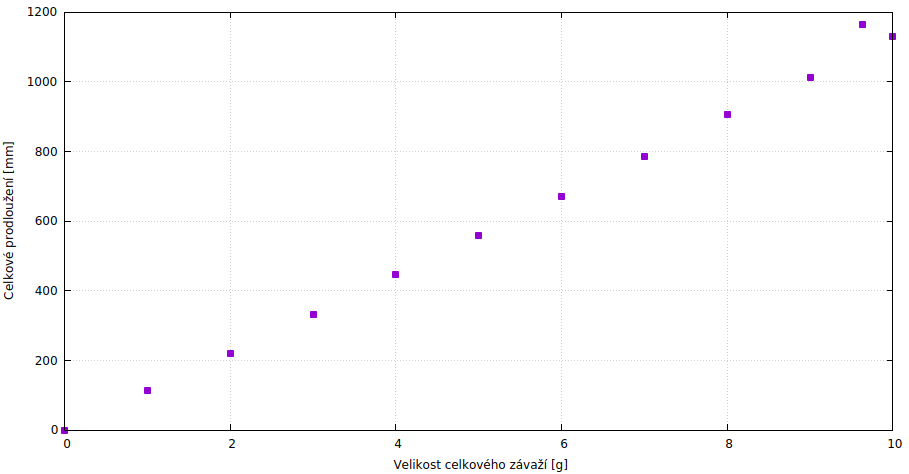
\includegraphics[width=0.8\textwidth]{mereni1.png}
            \caption{Měření prodloužení drátu v závěrslosti na celkovém zatížení}
            \label{fig:mereni1}
        \end{figure}

        \paragraph{} Fitování na linerání funkci ($f(x) = ax + b$) jsem provedl v 
        programu gnuplot s následujícím výsledkem.

        $$f(x) = 113.015x - 3.39723$$

        pro směrnici $a = 113.0, u(a) = 0.3$ platí

        \begin{equation}
            u(E) = \frac{4 g l}{\pi d^{2} a}
        \end{equation}

        \paragraph{} Pro odchylku ze ZŠN platí

        \begin{equation}
            u(E) = \frac{4 g l}{\pi d^{2} a} \sqrt{\left( \frac{2u(d)}{d} \right) ^{2} 
                + \left( \frac{u(a)}{a} \right) ^{2}}
        \end{equation}

        tedy výsledná nejistota modulu pružnosti je
        
        $$u(E) = 3490$$

        a po dosazení

        $$E = (173 \pm 3) kPa$$

    \subsection{Modul pružnosti v tahu z průhybu nosníku}

        \begin{table}[h]
            \centering
            \begin{tabular}{ | l | l || l | l | }
                \hline
                    mosaz (a [cm]) & mosaz (b [cm]) & ocel (a [cm]) & ocel (b [cm]) \\ \hline
                    0.510 & 2.835 & 0.485 & 2.845 \\ \hline
                    0.505 & 2.840 & 0.480 & 2.855 \\ \hline
                    0.505 & 2.840 & 0.485 & 2.845 \\ \hline
                    0.525 & 2.830 & 0.480 & 2.840 \\ \hline
                    0.500 & 2.835 & 0.480 & 2.840 \\ \hline
                    0.520 & 2.840 & 0.485 & 2.840 \\ \hline
                    0.510 & 2.845 & 0.485 & 2.830 \\ \hline
                    0.500 & 2.850 & 0.490 & 2.840 \\ \hline
                    0.510 & 2.840 & 0.485 & 2.845 \\ \hline
                    0.505 & 2.840 & 0.470 & 2.855 \\
                \hline
            \end{tabular}
            \caption{Rozměry nosníku}
            \label{fig:rozmery}
        \end{table}

        \paragraph{} Nejprve jsem změřil rozměry nosníků 

        $$a_{mosaz} = (0.51 \pm 0.05) mm$$
        $$b_{mosaz} = (2.84 \pm 0.05) mm$$
        $$l_{mosaz} = (90.1 \pm 0.1) mm$$
        $$a_{ocel} = (0.48 \pm 0.05) mm$$
        $$b_{ocel} = (2.84 \pm 0.05) mm$$
        $$l_{ocel} = (90.1 \pm 0.1) mm$$
        
        \begin{figure}[h]
            \centering
            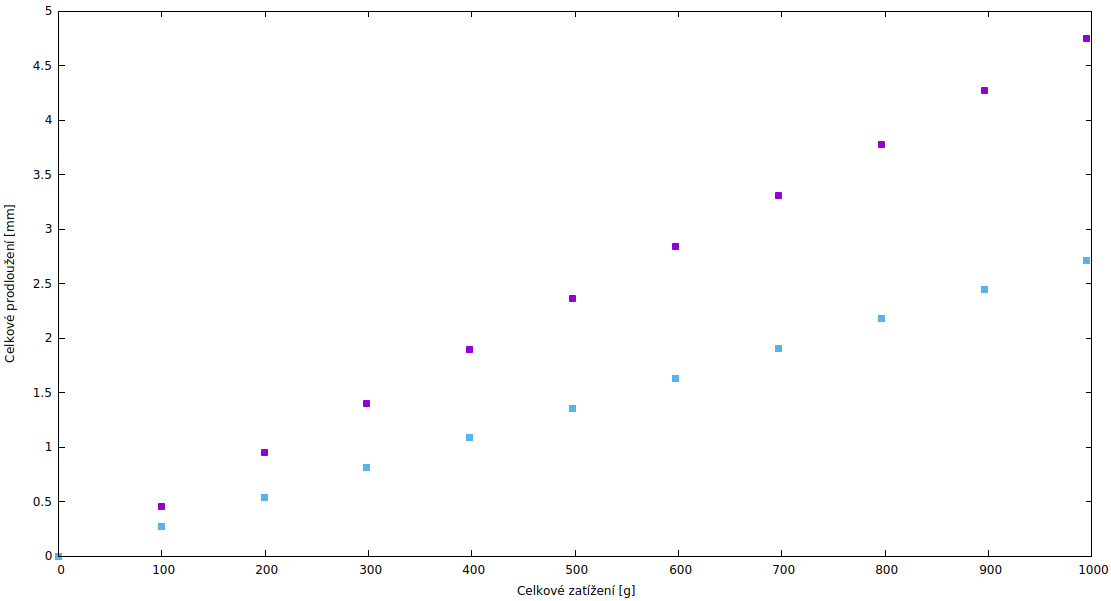
\includegraphics[width=0.8\textwidth]{mereni2.png}
            \caption{Měření prohnutí desek v závislosti na zatížení. Fialové body = mosaz. 
                Modré body = ocel}
            \label{fig:mereni2}
        \end{figure}

        \paragraph{} Podobně jako u prvního měření si nechám programem gnuplot vypočítat
            lineární regresy a zjistím parametr $y$ z rovnice níže.

        \begin{equation}
            E = \frac{m g l^{3}}{4 a^{3} b y}
        \end{equation}

        $$y_{mosaz} = 0.0047733 \pm 9.441 \cdot 10 ^{-6}$$
        $$y_{ocel} = 0.00273151 \pm 2.145 \cdot 10 ^{-6}$$

        \paragraph{} Ze ZŠN určím nejistotu $měření pomocí vzorce níže$.

        \begin{equation}
            u(E) = \frac{g l^{3}}{4 a^{3} b y} \sqrt{\left( \frac{3u(l)}{l} \right) ^{2} 
                + \left( \frac{ 3 u(a)}{a} \right) ^{2}
                + \left( \frac{u(b)}{b} \right) ^{2} 
                + \left( \frac{u(y)}{y} \right) ^{2} }
        \end{equation}

        po dosazení

        $$E_{mosaz} = (10.0 \pm 0.3) MPa$$
        $$E_{ocel} = (197.0 \pm 0.6) MPa$$

    \subsection{Modul pružnosti ve smyku}

        \paragraph{}

        $$ l = 52.2 cm $$
        $$ m = (1.99 \pm 0.01) cm $$

        \begin{equation}
            G = \frac{16 \pi m R^{2} l}{5 r^{4} T^{2}}
        \end{equation}

        \paragraph{} Nejistotu měření určím pomocí

        \begin{equation}
            u(G) = G \sqrt{\left( \frac{2 u(R)}{R} \right)^{2} + \left( \frac{u(l)}{l} \right)^{2} + \left( \frac{4 u(r)}{r} \right)^{2} 
                + \left( \frac{2 u(T)}{T} \right)^{2}}
        \end{equation}

        \paragraph{} což po dosazení dává výsledek

        $$G = (136 \pm 3) GPa$$

    \section{Zhodnocení měření, závěr}

    \paragraph{} Při měření byl použit multimetr s relativní přesností $0.1\%$ při měření napětí
        a $0,3\%$, resp. $0.8\%$ při měření proudu do rozsahu $400 mA$, resp. $4 mA$. Výsledky 
        měření jsou shrnuty v tabulce 3.
\end{document}

